\documentclass[aspectratio=169]{beamer}

\mode<presentation>

\usepackage[utf8]{inputenc}
\usepackage[T1]{fontenc}	%makes å,ä,ö etc. proper symbols
\usepackage{amsmath}
\usepackage{graphicx}
\usepackage{xcolor}
\usepackage{listings}
\usepackage{multicol}
\usepackage{hyperref}

\usepackage{tikz}
\usepackage{forest}
\usetikzlibrary{shapes}


\definecolor{LundaGroen}{RGB}{00,68,71}
\definecolor{StabilaLila}{RGB}{85,19,78}
\definecolor{VarmOrange}{RGB}{237,104,63}

\definecolor{MagnoliaRosa}{RGB}{251,214,209}
\definecolor{LundaHimmel}{RGB}{204,225,225}
\definecolor{LundaLjus}{RGB}{255,242,191}

\usefonttheme{serif}
\usetheme{malmoe}
\setbeamercolor{palette primary}{bg=VarmOrange}
\setbeamercolor{palette quaternary}{bg=LundaGroen}
\setbeamercolor{background canvas}{bg=LundaLjus}
\setbeamercolor{structure}{fg=LundaGroen}

\usepackage[many]{tcolorbox}

\newtcolorbox{cross}{blank,breakable,parbox=false,
  overlay={\draw[red,line width=5pt] (interior.south west)--(interior.north east);
    \draw[red,line width=5pt] (interior.north west)--(interior.south east);}}



\lstset{language=Python} 
\lstset{%language=[LaTeX]Tex,%C++,
    morekeywords={PassOptionsToPackage,selectlanguage,True,False},
    keywordstyle=\color{blue},%\bfseries,
    basicstyle=\small\ttfamily,
    %identifierstyle=\color{NavyBlue},
    commentstyle=\color{red}\ttfamily,
    stringstyle=\color{VarmOrange},
    numbers=left,%
    numberstyle=\scriptsize,%\tiny
    stepnumber=1,
    numbersep=8pt,
    showstringspaces=false,
    breaklines=true,
    %frameround=ftff,
    frame=single,
    belowcaptionskip=.75\baselineskip,
	tabsize=4,
	backgroundcolor=\color{white}
    %frame=L
}

\begin{document}

\lstset{literate=
  {á}{{\'a}}1 {é}{{\'e}}1 {í}{{\'i}}1 {ó}{{\'o}}1 {ú}{{\'u}}1
  {Á}{{\'A}}1 {É}{{\'E}}1 {Í}{{\'I}}1 {Ó}{{\'O}}1 {Ú}{{\'U}}1
  {à}{{\`a}}1 {è}{{\`e}}1 {ì}{{\`i}}1 {ò}{{\`o}}1 {ù}{{\`u}}1
  {À}{{\`A}}1 {È}{{\'E}}1 {Ì}{{\`I}}1 {Ò}{{\`O}}1 {Ù}{{\`U}}1
  {ä}{{\"a}}1 {ë}{{\"e}}1 {ï}{{\"i}}1 {ö}{{\"o}}1 {ü}{{\"u}}1
  {Ä}{{\"A}}1 {Ë}{{\"E}}1 {Ï}{{\"I}}1 {Ö}{{\"O}}1 {Ü}{{\"U}}1
  {â}{{\^a}}1 {ê}{{\^e}}1 {î}{{\^i}}1 {ô}{{\^o}}1 {û}{{\^u}}1
  {Â}{{\^A}}1 {Ê}{{\^E}}1 {Î}{{\^I}}1 {Ô}{{\^O}}1 {Û}{{\^U}}1
  {œ}{{\oe}}1 {Œ}{{\OE}}1 {æ}{{\ae}}1 {Æ}{{\AE}}1 {ß}{{\ss}}1
  {ű}{{\H{u}}}1 {Ű}{{\H{U}}}1 {ő}{{\H{o}}}1 {Ő}{{\H{O}}}1
  {ç}{{\c c}}1 {Ç}{{\c C}}1 {ø}{{\o}}1 {å}{{\r a}}1 {Å}{{\r A}}1
  {€}{{\euro}}1 {£}{{\pounds}}1 {«}{{\guillemotleft}}1
  {»}{{\guillemotright}}1 {ñ}{{\~n}}1 {Ñ}{{\~N}}1 {¿}{{?`}}1
}

% NEW COMMANDS
\newcommand{\fortt}{\texttt{for}}
\newcommand{\whilett}{\texttt{while}}
\newcommand{\iftt}{\texttt{if}}

\AtBeginSection[ ]
{
\begin{frame}{Outline}
    \tableofcontents[currentsection]
\end{frame}
}

\title{Binära träd}
\date{vt 24}
\author{Programmering 2}

\maketitle

\tableofcontents

\section{Trädstrukturer}

\begin{frame}
	\frametitle{Träd}
	\centering
	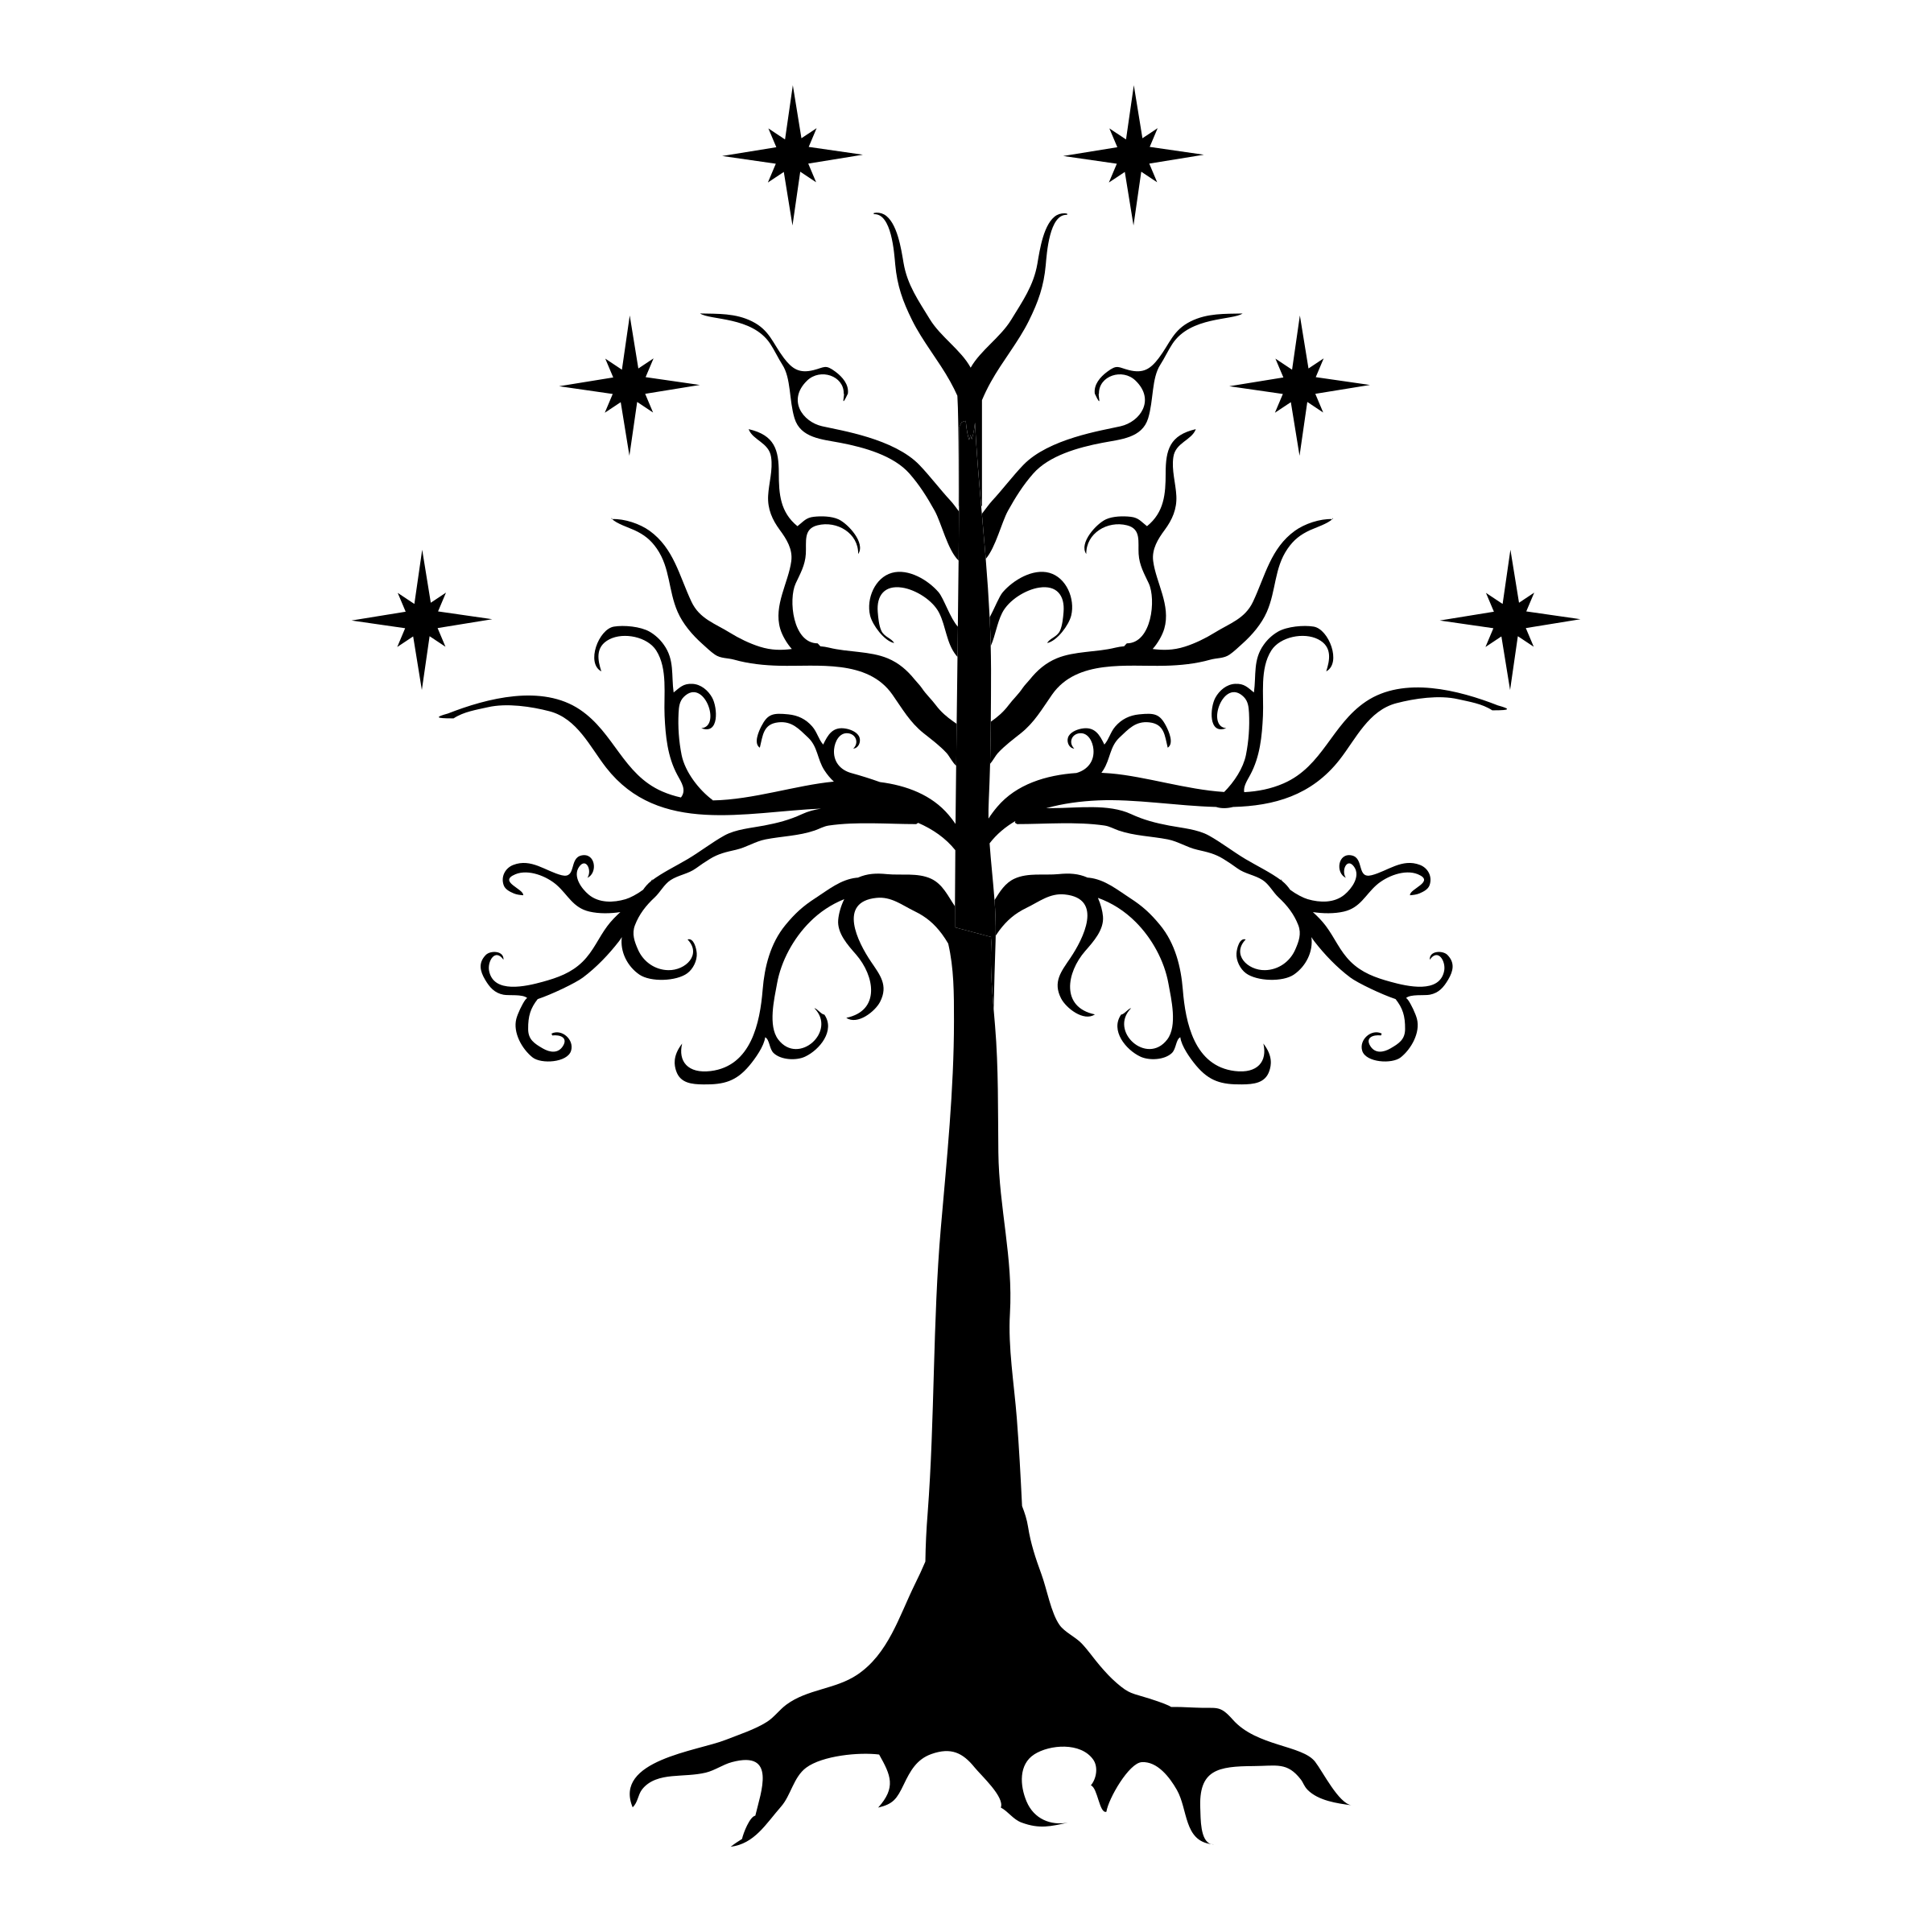
\includegraphics[width=.45\linewidth]{tree-of-gondor.png}
	
\end{frame}

\begin{frame}
	\frametitle{Träd}
	\begin{itemize}
		\item När vi pratar om datastrukturen träd så brukar den vara upp-och-ner
	\end{itemize} 
	\centering
	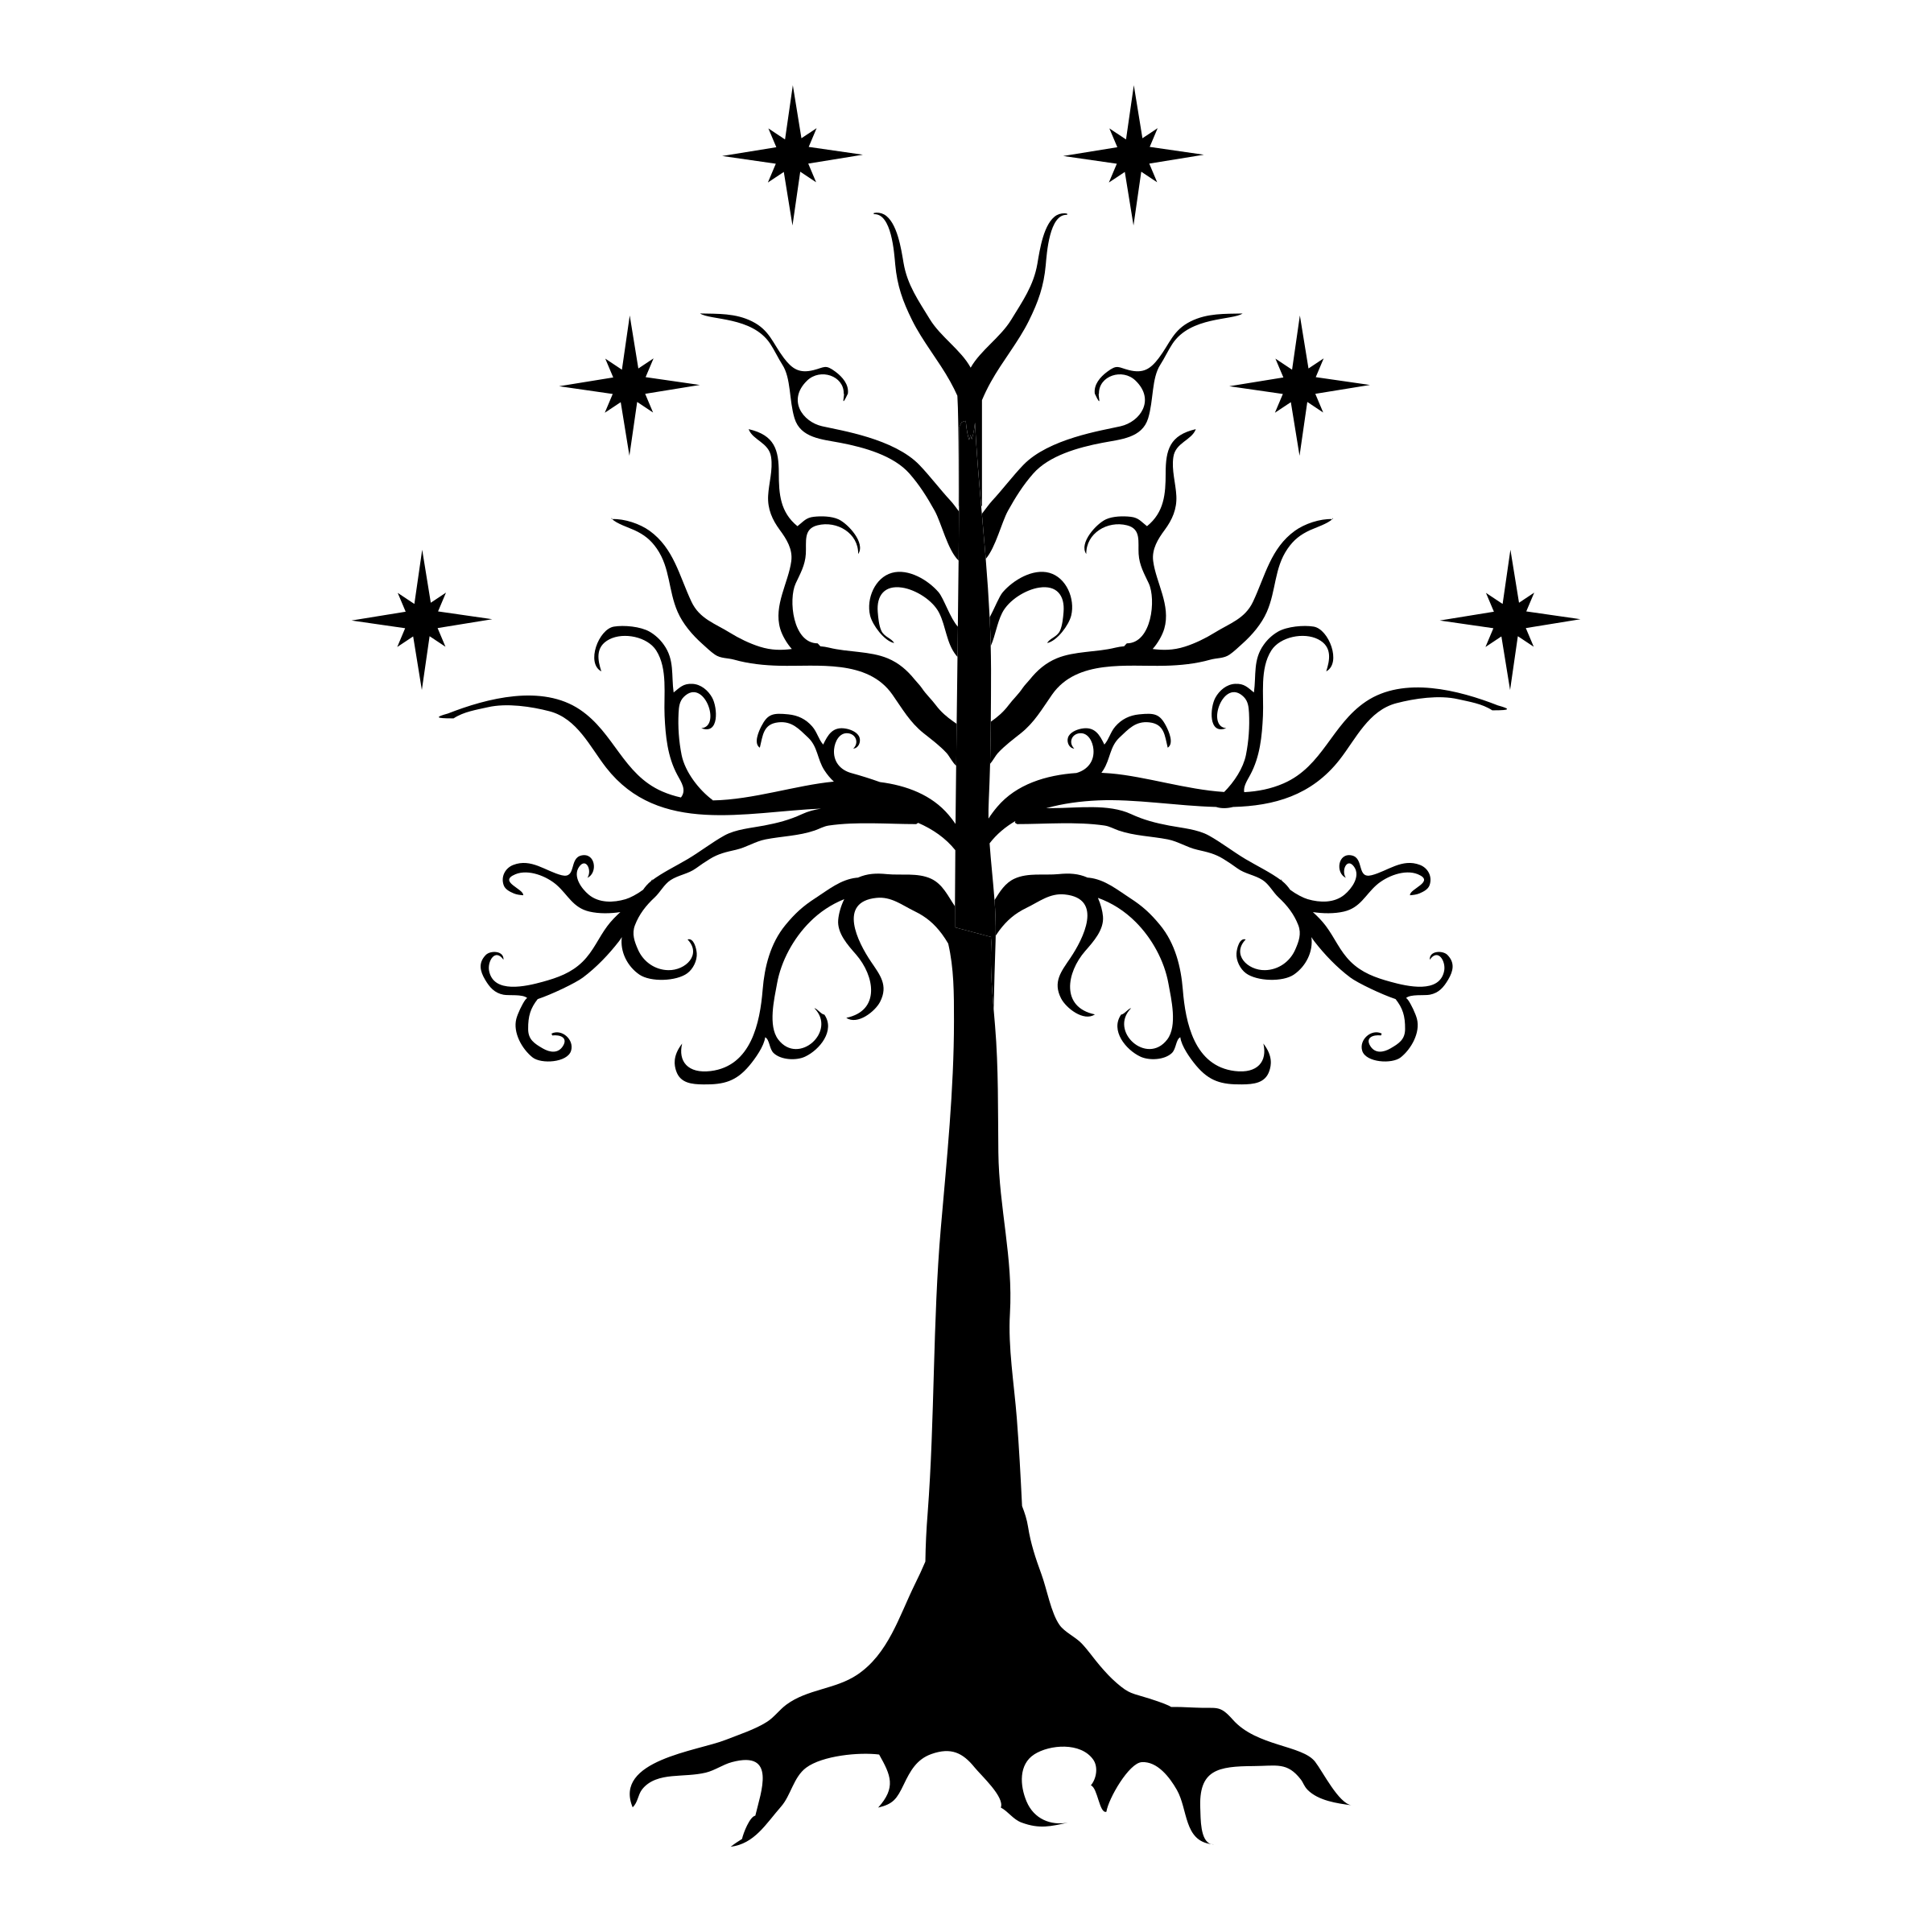
\includegraphics[width=.45\linewidth,angle=180,origin=c]{tree-of-gondor.png}	
\end{frame}

\subsection{Exempel}

\begin{frame}
	\frametitle{Träd}
	\framesubtitle{Släktträd}
	
	
	\begin{itemize}
		\item Träd används inte bara inom programmering, utan för att visa annan data också
	\end{itemize}
	
	\centering
	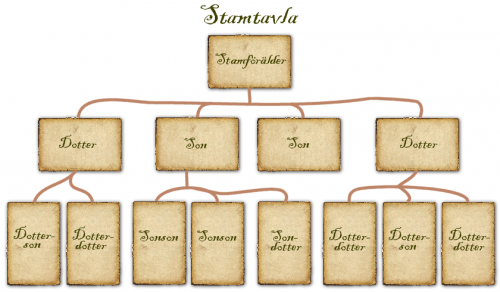
\includegraphics[width=.65\linewidth]{Stamtavla.png}
	
\end{frame}

\begin{frame}
	\frametitle{Träd}
	\framesubtitle{Utfallsdiagram}
	
	\begin{itemize}
		\item I Matematik 1 gjorde vi träd i sannolikheten
	\end{itemize}
	
	\centering
	\begin{forest}
		[ljussignal
			[grönt
				[grönt]
				[rött]
			]
			[rött
				[grönt]
				[rött]
			]
		]
	\end{forest}
	
	
\end{frame}

\section{Binära träd}

\begin{frame}
	\frametitle{Binära träd}

	\begin{itemize}
		\item Ett binärt träd är ett träd där varje nod har högst två barn
	\end{itemize}
	
	\centering
	\begin{forest}
		[8
			[4
				[2
					[1]
					[3]
				]
				[6
					[5]
					[7]
				]
			]
			[12
				[10
					[9]
					[11]
				]
				[14
					[13]
					[15]
				]
			]
		]
	\end{forest}

\end{frame}

\begin{frame}
	\frametitle{Binära träd}
	\framesubtitle{Balanserade träd}
	
	\begin{itemize}
		\item Träd kan vara balanserade, eller obalanserade
	\end{itemize}
	
	\begin{center}
		\begin{tabular}{cc}
		\begin{forest}
			[4
				[2
					[1]
					[3]
				]
				[6
					[5]
					[7]
				]
			]
		\end{forest}
		&
		\begin{forest}
			[5
				[2
					[1]
					[3
						[4]
					]
				]
				[6
					[7]
				]
			]
		\end{forest}
		\end{tabular}
	\end{center}
	
\end{frame}

\begin{frame}
	\frametitle{Binära träd}
	\framesubtitle{Att hitta i ett binärt träd}
	
	\begin{itemize}
		\item När du ska hitta i ett binärt träd så börjar du med den översta noden.
		\item Om det är elementet du letar efter är du klar
		\item Annars går du letar efter ett större tal och till vänster om ditt tal är mindre
		\item Den här processen upprepas tills du har hittat rätt.
	\end{itemize}
	
	Tidskomplexitet för att hitta rätt plats i ett binärt träd är \(O(log_2{(n)})\) (i en länkad lista är tidskomplexiteten \(O(n)\)), du behöver alltså göra ungefär tre kontroller om det finns åtta element i listan (\(2^3=8\)) och bara tio kontroller om det finns 1000 element i listan (\(2^{10}=1024\)).
	
\end{frame}

\begin{frame}
	\frametitle{Binära träd}
	\framesubtitle{Skapa ett träd}
	
	\begin{itemize}
		\item Säg att du vill skapa ett träd som innehåller talen: 5, 3, 2, 4, 7, 6, 8, 1 (och att du får talen i den ordningen)
		\item Först stoppar du in 5 överst
	\end{itemize}
	
	\centering
	\begin{forest}
		[5]
	\end{forest}

\end{frame}

\begin{frame}
	\frametitle{Binära träd}
	\framesubtitle{Skapa ett träd}
	
	\begin{itemize}
		\item Säg att du vill skapa ett träd som innehåller talen: 5, 3, 2, 4, 7, 6, 8, 1 (och att du får talen i den ordningen)
		\item Sen ska 3 in till vänster
	\end{itemize}
	
	\centering
	\begin{forest}
		[5 [3]]
	\end{forest}

\end{frame}

\begin{frame}
	\frametitle{Binära träd}
	\framesubtitle{Skapa ett träd}
	
	\begin{itemize}
		\item Säg att du vill skapa ett träd som innehåller talen: 5, 3, 2, 4, 7, 6, 8, 1 (och att du får talen i den ordningen)
		\item Sen är 2 mindre än 5 och mindre än 3. Så den ska till vänster om 5 och vänster om 3
	\end{itemize}
	
	\centering
	\begin{forest}
		[5 [3 [2]]]
	\end{forest}

\end{frame}

\begin{frame}
	\frametitle{Binära träd}
	\framesubtitle{Skapa ett träd}
	
	\begin{itemize}
		\item Säg att du vill skapa ett träd som innehåller talen: 5, 3, 2, 4, 7, 6, 8, 1 (och att du får talen i den ordningen)
		\item Sen är 4 mindre än 5 och större än 3. Så den ska till vänster om 5 och höger om 3
	\end{itemize}
	
	\centering
	\begin{forest}
		[5 [3 [2] [4]]]
	\end{forest}

\end{frame}

\begin{frame}
	\frametitle{Binära träd}
	\framesubtitle{Skapa ett träd}
	
	\begin{itemize}
		\item Säg att du vill skapa ett träd som innehåller talen: 5, 3, 2, 4, 7, 6, 8, 1 (och att du får talen i den ordningen)
		\item Sen är 7 större än 5. Så den ska till höger om 5
	\end{itemize}
	
	\centering
	\begin{forest}
		[5 [3 [2] [4]] [7]]
	\end{forest}

\end{frame}

\begin{frame}
	\frametitle{Binära träd}
	\framesubtitle{Skapa ett träd}
	
	\begin{itemize}
		\item Säg att du vill skapa ett träd som innehåller talen: 5, 3, 2, 4, 7, 6, 8, 1 (och att du får talen i den ordningen)
		\item Sen är 6 större än 5 och mindre än 7. Så den ska till höger om 5 och till vänster om 7
	\end{itemize}
	
	\centering
	\begin{forest}
		[5 [3 [2] [4]] [7 [6]]]
	\end{forest}

\end{frame}

\begin{frame}
	\frametitle{Binära träd}
	\framesubtitle{Skapa ett träd}
	
	\begin{itemize}
		\item Säg att du vill skapa ett träd som innehåller talen: 5, 3, 2, 4, 7, 6, 8, 1 (och att du får talen i den ordningen)
		\item Sen är 8 större än 5 och större än 7. Så den ska till höger om 5 och till höger om 7
	\end{itemize}
	
	\centering
	\begin{forest}
		[5 [3 [2] [4]] [7 [6] [8]]]
	\end{forest}

\end{frame}

\begin{frame}
	\frametitle{Binära träd}
	\framesubtitle{Skapa ett träd}
	
	\begin{itemize}
		\item Säg att du vill skapa ett träd som innehåller talen: 5, 3, 2, 4, 7, 6, 8, 1 (och att du får talen i den ordningen)
		\item Sen är 1 mindre än 5, mindre än 3 och mindre än 2. Så den ska till vänster om 5, till vänster om 3 och till vänster om 2.
	\end{itemize}
	
	\centering
	\begin{forest}
		[5 [3 [2 [1]] [4]] [7 [6] [8]]]
	\end{forest}

\end{frame}

\begin{frame}
	\frametitle{Binära träd}
	\framesubtitle{Skapa ett träd}
	
	\begin{itemize}
		\item Säg att du ändrar ordningen talen kommer i till: 2, 6, 4, 1, 3, 7, 8, 5 
		\item Då hade trädet sett ut så här istället:
	\end{itemize}
	
	\centering
	\begin{forest}
		[2 [1] [6 [4 [3]] [7 [5][8]]]]
	\end{forest}

\end{frame}

\section{Noden}

\begin{frame}[fragile]
	\frametitle{Noden}

	\begin{itemize}
		\item Klassen \texttt{Node} behöver se lite annorlunda ut jämfört med hur den ser ut för strukturerna \texttt{Stack} och \texttt{Queue}.
		\item \texttt{Node} behöver \textit{peka} till två element, elementet till höger och elementet till vänster
	\end{itemize}
	
	\begin{lstlisting}
class Node():
    def __init__(self, value):
        self.value = value
        self.left = None
        self.right = None
	\end{lstlisting}
	
\end{frame}

\section{Övningar}

\begin{frame}
	\frametitle{Övningar}
	
	\begin{enumerate}
		\item Börja med att skapa ett träd för hand, med papper och penna. Skapa ett träd av talen: 5, 3, 11, 6, 13, 8, 2, 4, 1, 10, 14, 15, 9, 12, 7
		\item Skapa klassen \texttt{Node}
		\item Skapa också klassen \texttt{BinaryTree} som kan ta emot nya tal
	\end{enumerate}
	
\end{frame}

\end{document}